\documentclass[../../main.tex]{subfiles}
\begin{document}

\begin{flushright}
  \footnotesize\textit{【自動文字起こし・要確認】}
\end{flushright}

{\bf [解]}
\textbf{(p)} 正$n$角形の頂点を左から$A_1,\ldots,A_n$とする．$\angle A_lA_2A_m$（$l<m$）が$60^\circ$に等しい時，正$n$角形は円に内接することと円周角の定理から，$l=2$の時を考えれば良い．正$n$角形の内接する円の中心を$O$とし，この半径を$1$として良い．$\triangle A_1A_2A_m$に正弦定理を用いて，
\begin{figure}[H]
  \centering
  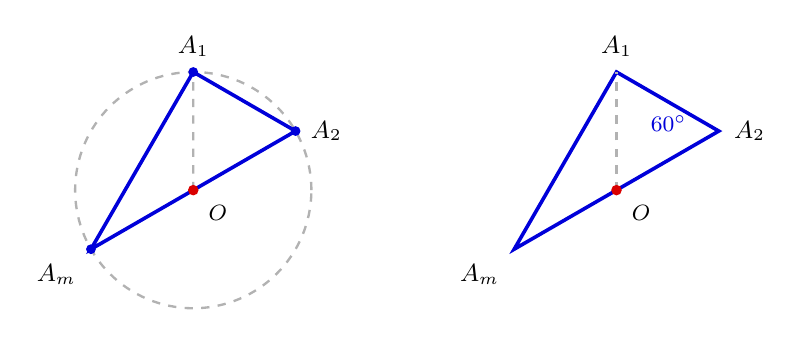
\begin{tikzpicture}[scale=1.25, >=stealth,
    every node/.style={font=\small}]
    % 手書きの円と三角形を，n=6, m=5 の具体例で並べて示す．
    \begin{scope}
      \coordinate (O) at (0,0);
      \coordinate (Aone) at (90:1.2);
      \coordinate (Atwo) at (30:1.2);
      \coordinate (Am) at (210:1.2);
      \draw[dashed, gray!60, line width=0.85pt] (O) circle (1.2);
      \draw[dashed, gray!60, line width=0.8pt] (O)--(Aone) (O)--(Am);
      \draw[blue!85!black, line width=1.3pt]
      (Aone)--(Atwo)--(Am)--cycle;
      \node[circle, fill=red!85!black, inner sep=1.35pt] at (O) {};
      \node[below right=2pt, font=\footnotesize] at (O) {$O$};
      \foreach \point/\position/\name in {
      Aone/above/$A_1$, Atwo/right/$A_2$, Am/below left/$A_m$} {
        \node[circle, fill=blue!85!black, inner sep=1.25pt] at (\point) {};
        \node[\position=2pt] at (\point) {\name};
      }
    \end{scope}
    \begin{scope}[xshift=4.3cm]
      \coordinate (Aone2) at (0,1.2);
      \coordinate (Atwo2) at (1.03923,0.6);
      \coordinate (Am2) at (-1.03923,-0.6);
      \coordinate (O2) at (0,0);
      \draw[blue!85!black, line width=1.3pt]
      (Aone2)--(Atwo2)--(Am2)--cycle;
      \draw[dashed, gray!60, line width=0.8pt]
      (O2)--(Aone2);
      \node[circle, fill=red!85!black, inner sep=1.35pt] at (O2) {};
      \node[below right=2pt, font=\footnotesize] at (O2) {$O$};
      \node[above=2pt] at (Aone2) {$A_1$};
      \node[right=2pt] at (Atwo2) {$A_2$};
      \node[below left=2pt] at (Am2) {$A_m$};
      \node[font=\footnotesize, blue!85!black] at (0.53,0.68) {$60^\circ$};
    \end{scope}
  \end{tikzpicture}
  \caption{円周角$\angle A_1A_2A_m=60^\circ$と弦$A_1A_m$（$n=6,m=5$の例）}
\end{figure}
\begin{align}
  \dfrac{|A_1A_m|}{\sin60^\circ}=2\quad\therefore\ |A_1A_m|=\sqrt{3}\quad\cdots①
\end{align}

一方，$\angle A_1OA_m=2\pi\dfrac{n-m+1}{n}$だから，
\begin{align}
  |A_1A_m|=2\sin\pi\dfrac{n-m+1}{n}\quad\cdots②
\end{align}

①，②から
\begin{align}
  \sin\dfrac{n-m+1}{n}\pi&=\dfrac{\sqrt{3}}{2}\\
  \sin\left(\pi-\dfrac{m-1}{n}\pi\right)&=\dfrac{\sqrt{3}}{2}\\
  \sin\dfrac{m-1}{n}\pi&=\dfrac{\sqrt{3}}{2}
\end{align}

$3\le m\le n$から，$0<\dfrac{m-1}{n}<1$だから，
\begin{align}
  \dfrac{m-1}{n}\pi=\dfrac{1}{3}\pi,\ \dfrac{2}{3}\pi
\end{align}
\begin{align}
  n=3(m-1)\quad\text{or}\quad n=3\cdot\dfrac{m-1}{2}
\end{align}

$m\in\mathbb N$及びいずれの場合も，$n$は$3$の倍数である．よって(p)は正しい．

\textbf{(q)} 下図のような正六角形内に$A$，$B$，$C$，$D$をとる．この時，(p)の議論から，
\begin{align}
  \angle ACB=\angle ADB\quad\cdots③
\end{align}
であり，かつ
\begin{align}
  |AC|<|AD|，\quad|BC|<|BD|\quad\cdots④
\end{align}
となる．したがって，③，④から，このような4点$A,B,C,D$は(q)の反例となる．よって(q)は正しくない．

\begin{figure}[H]
  \centering
  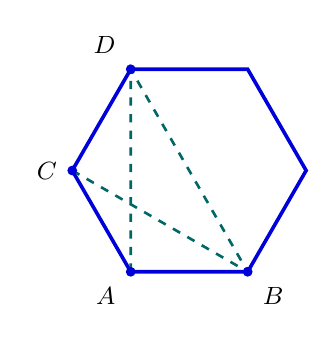
\begin{tikzpicture}[scale=1.1, >=stealth,
    every node/.style={font=\small}]
    \foreach \i in {0,...,5} {
      \coordinate (V\i) at ({180-60*\i}:1.35);
    }
    % C は左，D は左上，A,B は下辺の両端．
    \draw[blue!85!black, line width=1.3pt]
    (V0)--(V1)--(V2)--(V3)--(V4)--(V5)--cycle;
    \draw[dashed, teal!80!black, line width=0.95pt]
    (V0)--(V4) (V5)--(V1)--(V4);
    \foreach \point/\position/\name in {
      V0/left/$C$, V1/above left/$D$,
    V5/below left/$A$, V4/below right/$B$} {
      \node[circle, fill=blue!85!black, inner sep=1.25pt] at (\point) {};
      \node[\position=2pt] at (\point) {\name};
    }
  \end{tikzpicture}
  \caption{正六角形内の点$A$，$B$，$C$，$D$（(q)の反例）}
\end{figure}

\newpage

\end{document}
